% !TEX encoding = UTF-8 Unicode
% -*- coding: UTF-8; -*-
% vim: set fenc=utf-8
\documentclass[a4paper,12pt,french]{article}

\usepackage{centrale}

\hypersetup{
    pdftitle={Rapport synthèse lot 1},
    pdfauthor={},
    pdfsubject={PE-01 Apprentissage automatique pour la discrétisation des lois de conservation},
    pdfproducer={Conversion PDF à insérer},
    pdfkeywords={} %
}

\DeclareGraphicsRule{.ai}{pdf}{.ai}{} % pour insérer des documents .ai
\graphicspath{ {./img/} {./eps/}} % pour ne pas avoir à ajouter eps/ton-image.jpg

% ------------- Packages spéciaux, nécessaires pour ce rapport, à insérer ici ------------- 


\begin{document}

% --------------------------------------------------------------
%                       Page de garde
% --------------------------------------------------------------

\begin{titlepage}
\begin{center}

\includegraphics[width=1\textwidth]{logo_ECL_rectangle_quadri_vectoriel.ai}\\[1cm]

{\large PE-01 Apprentissage automatique pour la discrétisation des lois de conservation}\\[0.5cm]

% Title
\rule{\linewidth}{0.5mm} \\[0.4cm]
{ \huge \bfseries Rapport de synthèse lot 1 \\[0.4cm] }
\rule{\linewidth}{0.5mm} \\[1.5cm]

% Author and supervisor
\noindent
\begin{minipage}{0.5\textwidth}
  \begin{flushleft} \large
    \emph{Auteurs :}\\
    M. Vicente \textsc{Cittolin}\\
    M. Sebastián \textsc{Flores}\\
    M. Jonathan \textsc{Guérin}\\
    Mme. Clémence \textsc{Martin}\\
    M. Abderrahmane \textsc{Rachadi}\\
    M. Hugo \textsc{Tosello}
  \end{flushleft}
\end{minipage}%
\begin{minipage}{0.5\textwidth}
  \begin{flushright} \large
    \emph{Tuteurs :} \\
    M.~Alexis \textsc{Giauque}\\
    M.~Cristophe \textsc{Corre}
  \end{flushright}
\end{minipage}

\vfill

% Bottom of the page
{\large Version du\\ \today}

\end{center}
\end{titlepage}

% --------------------------------------------------------------
%                    Table des matières 
% --------------------------------------------------------------

%\thispagestyle{empty}
%\tableofcontents
%\newpage

% --------------------------------------------------------------
%                         Partie 1
% --------------------------------------------------------------

\section{Description des tâches réalisées}
Tout d'abord, on a transcrit le code SciLab pour la discrétisation
de l'équation de diffusion en 1D dans le langage Python. \'Etant une 
tâche initiale de prise en main, aucun problème notable n'a été 
rencontré.
\\

L'objectif de ce lot est de réaliser un réseau de neurones capable
de donner un pas de temps $dt$ maximal pour une paire de paramètres
$\alpha$ et $dx$ donnée. De ce fait, on s'est mis à créer (i) une 
base de données de simulation du problème et (ii) un algorithme
de création et entraînement d'un réseau de neurones.
\\

Pour la création de la base de données, on a écrit un algorithme Python
pour la générer, et on la sauvegarde en format SQL (extension \textit{.db}).
Le premier problème rencontré est le temps de calcul pris par l'algorithme,
ce qui demande de diviser l'exécution du programme en deux 
ordinateurs et la tâche postérieur de consolider les deux bases
générées dans un seul fichier \textit{.db}.
\\

Pour le réseau de neurones, et après avoir résolu les problèmes
d'installation du module TensorFlow sur les ordinateurs de toute l'équipe,
le codage de l'algorithme d'entraînement est réalisé sans problèmes majeurs. La fonction d'activation est d'abord ReLU et on expérimente avec différentes nombres de couches et de neurones par couche.
A priori, les résultats d'entraînement sont satisfaisants, c'est-à-dire, on
obtient des paramètres de correlation et de $R^2$ bien proches de 1.
\\

Suite à la rencontre de plusieurs valeurs \textit{NaN} dans la 
base de données, on a trouvé des fautes dans l'algorithme qui
la génère. Après la correction de ces erreurs, une nouvelle base
de données est créée, cette fois-ci, avec plus de points. Le problème du temps de calcul est accentué, prenant plusieurs jours pour finir une partie. 
\\

Avant de l'entraînement du réseau, on ajoute un filtrage des données : on enlève les points qui ne sont pas stables et on prend les points avec la plus grande valeur de \textit{dt}. Ce processus-ci laisse la base de données d'une taille considérablement plus petite que à l'origine (environ $90\%$ des données sont enlevées).
\\

Pour diminuer le temps de calcul, le code de génération de base de données est traduit en C++, ce qui en effet rend l'exécution considérablement plus rapide, générant le même volume de données en quelques minutes.
\\

Avec la nouvelle base de données, le réseau est entraîné de nouveau, et un script est créé pour tester la performance par rapport aux attentes théoriques. Ce test est fait par la génération de valeurs aléatoires de $\alpha$ et $dx$, puis leur insertion au réseau comme \textit{input}, et après la comparaison du \textit{output} avec la relation théorique $dt\leq \frac{dx^2}{\alpha}$.
\\

Une difficulté rencontrée à ce stade est la question de la normalisation des données d'entrée. Comme le réseau est entraîné avec une base de données normalisée, c'est-à-dire, de moyenne $\mu=0$ et écart-type $\sigma=1$, les données d'entrée doivent s'adapter à la façon dont le réseau est entraîné. La question principale est si les données d'entrée doivent être elles mêmes normalisés, ou si elles doivent être transformées par la moyenne et l'écart-type de la base de données d'entraînement avant normalisation. La décision a favorisé la deuxième option.
\\

Postérieurement à la comparaison des résultats du réseau et ceux de la théorie, on a remarqué que plusieurs prédictions du réseau sont au-dessus de la courbe théorique, et donc sont instables. Ce problème est dû principalement à deux faits principales : d'un côté, il y a des données dans la base qui sont marquées "stables" tandis qu'elles ne vérifient pas la relation théorique, et d'autre côté, il n'y a aucun moyen de pénaliser le réseau s'il donne des prédictions instables.
\\

Pour régler le premier problème, on a appliqué un deuxième filtrage des données en utilisant la relation théorique, ce qui n'est pas idéal si on prend en compte qu'avoir une relation aussi explicite pour évaluer la pertinence d'un point de la base est assez rare (même pour l'advection 2D cela ne sera pas le cas). On présentera les résultats avec ces deux filtrages différents. Pour le deuxième problème, on n'a pas trouvé une solution.
\\
% --------------------------------------------------------------
%                            Partie 2
% --------------------------------------------------------------

\section{Présentation des résultats}
\subsection*{Description de la base de données}

La base de données générée contient 7500 points, pour lesquels on stocke la valeur de $\alpha$, de $dx$, de $dt$, si le schéma est stable avec ces valeurs, le nombre d'itérations réalisées $N_{iter}$, et l'erreur en moyenne quadratique par rapport à la solution exacte. Pour toutes ces données, on fixe un temps maximal de $dt \cdot N_{iter} = 500$.
\\

\begin{table}
\centering
\begin{tabular}{|c|c|c|c|c|c|}
\hline 
$\alpha$ & $dx$ & $dt$ & stable & $N_{iter}$ & erreur\\	 
\hline 
$2,35\cdot 10^{-4}$ & 0,010582 & 0,233290 & 1 & 2143 & $8,19\cdot 10^{-4}$ \\ 
\hline 
$2,35\cdot 10^{-4}$ & 0,010582 & 0,242621 & 0 & 2060 & $4,87\cdot 10^{26}$ \\ 
\hline 
$2,35\cdot 10^{-4}$ & 0,010582 & 0,251953 & 0 & 1984 & $1,99\cdot 10^{88}$ \\ 
\hline 
$2,35\cdot 10^{-4}$ & 0,010582 & 0,261284 & 0 & 1913 & $2,40\cdot 10^{141}$ \\ 
\hline 
$2,35\cdot 10^{-4}$ & 0,010582 & 0,270616 & 0 & 1847 & $1,00\cdot 10^{7}$ \\ 
\hline 
\end{tabular} 
\caption{Tail de la base de données avant filtrage}
\label{tab:tailraw}
\end{table}

On voit dans le tableau \ref{tab:tailraw} que pour chaque paire $(\alpha,dx)$ on obtient plusieurs valeurs de $dt$.

Dans la figure \ref{fig:graph-av-filtrage} on trace la valeur de $dt$ en fonction de la valeur théorique de $dt_{max}$, $\frac{dx^2}{\alpha}$. La ligne rouge représente la fonction identité.
\begin{figure}[ht!]
    \centering
    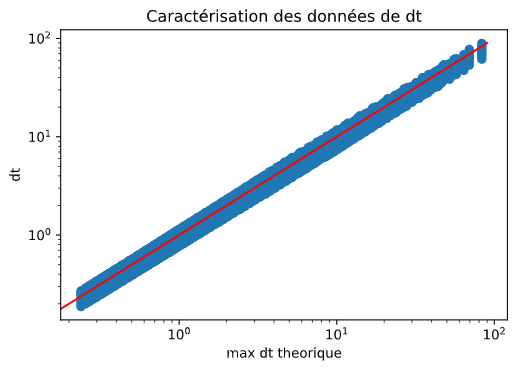
\includegraphics[width=0.8\textwidth]{base-av-filtrage.png}
    \caption{Graphique résumant la base de données avant filtrage en échelle log-log.}
    \label{fig:graph-av-filtrage}
\end{figure}

Pour la base de données filtrée, on obtient, dans les deux cas (filtrage avec et sans la relation théorique), une base de taille 750. Dans la figure \ref{fig:graph-apr-filtrage} on trace la même relation que dans la figure \ref{fig:graph-av-filtrage}, mais avec les deux bases filtrés. On peut bien voir que dans la base avec filtrage sans la relation théorique il existe un dépassement de la ligne de l'identité croissant à droite, ce qui veut dire que les données sont nommés stables par la base mais ne vérifient pas la relation $dt\leq \frac{dx^2}{\alpha}$. 
\\

\begin{figure}[ht!]
    \centering
    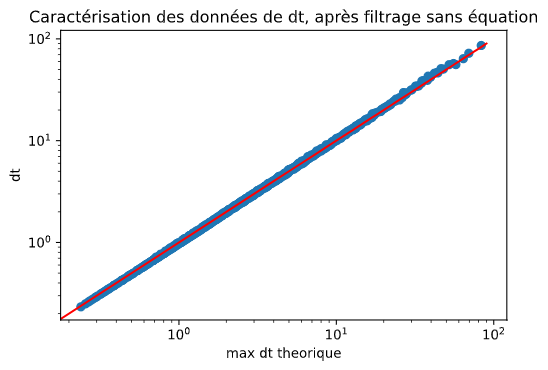
\includegraphics[width=0.70\textwidth]{base-apr-sanseq.png}
    \\
    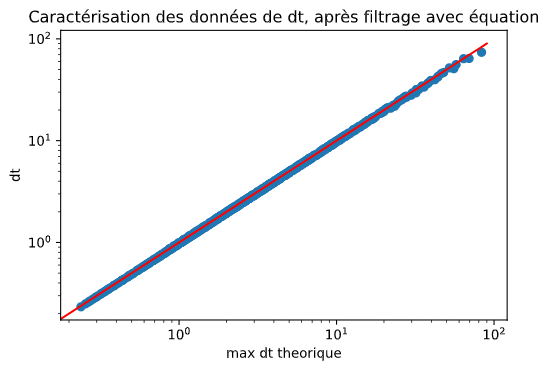
\includegraphics[width=0.70\textwidth]{base-apr-eq.png}
    \caption{Graphique résumant la base après filtrage sans équation (en haut), et avec l'équation (en bas).}
    \label{fig:graph-apr-filtrage}
\end{figure}

Dans la table \ref{tab:apresfiltre}, on peut voir les différences entre les paramètres des bases de données après filtrage. On note que dans le cas du filtrage avec équation, la moyenne et la valeur maximale de $dt$ sont plus basses.
\\

\begin{table}
\centering
\begin{tabular}{|c|c|c|c|}
\hline 
Sans équation & $\alpha$ & $dx$ & $dt$ \\ 
\hline 
Moyenne & $7,37\cdot 10^{-5}$ & $1,98\cdot 10^{-2}$ & $6,03$ \\ 
\hline 
Ecart-type & $5,61\cdot 10^{-5}$ & $8,71\cdot 10^{-3}$ & $9,26 $\\ 
\hline 
Maximum & $2,35\cdot 10^{-4}$ & $4,08\cdot 10^{-2}$ & $8,61\cdot 10$ \\ 
\hline 
Minimum & $1,00\cdot 10^{-5}$ & $1,06\cdot 10^{-2}$ & $2,33\cdot 10^{-1}$ \\ 
\hline 
\end{tabular}

\begin{tabular}{|c|c|c|c|}
\hline 
Avec équation & $\alpha$ & $dx$ & $dt$ \\ 
\hline 
Moyenne & $7,37\cdot 10^{-5}$ & $1,98\cdot 10^{-2}$ & $5,74$ \\ 
\hline 
Ecart-type & $5,61\cdot 10^{-5}$ & $8,71\cdot 10^{-3}$ & $9,26 $\\ 
\hline 
Maximum & $2,35\cdot 10^{-4}$ & $4,08\cdot 10^{-2}$ & $7,38\cdot 10$ \\ 
\hline 
Minimum & $1,00\cdot 10^{-5}$ & $1,06\cdot 10^{-2}$ & $2,33\cdot 10^{-1}$ \\ 
\hline 
\end{tabular}
\caption{Tableaux avec un résumé des deux bases de données après filtrage}
\label{tab:apresfiltre}
\end{table}

\subsection*{Résultats du réseau entraîné}

\begin{table}
\centering
\begin{tabular}{|ccc|}
\hline 
Type de couche & Output shape & N° paramètres \\ 
\hline 
\hline
Dense & (None, 5) & 15 \\ 
\hline 
LeakyReLU & (None, 5) & 0 \\ 
\hline 
Dense & (None, 20) & 120 \\ 
\hline 
LeakyReLU & (None, 20) & 0 \\ 
\hline 
Dense & (None, 20) & 420 \\ 
\hline 
LeakyReLU & (None, 20) & 0 \\ 
\hline 
Dense & (None, 1) & 21 \\ 
\hline 
\end{tabular} 
\caption{Structure du réseau de neurones}
\label{tab:struct}
\end{table}

Pour chacune des bases, nous avons entraîné le réseau avec les mêmes caractéristiques initiales, affichées dans la table \ref{tab:struct}. Le nombre de degrés de liberté est de 576.
\\

\begin{figure}[ht!]
    \centering
    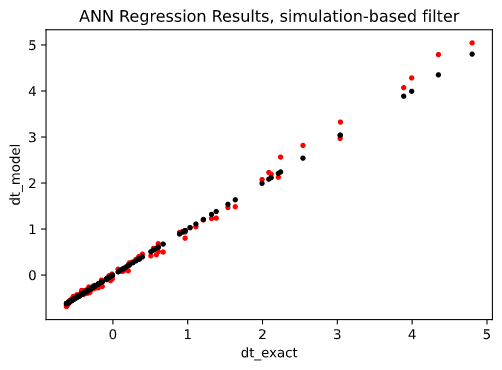
\includegraphics[width=0.45\textwidth]{results-simul.png}
    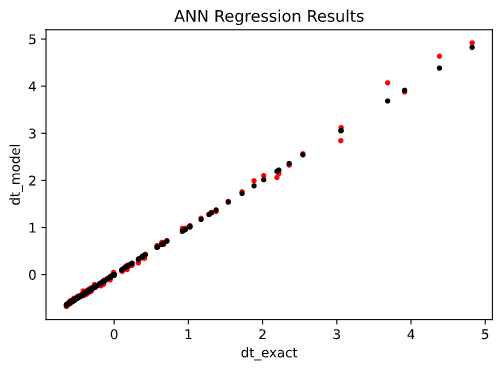
\includegraphics[width=0.45\textwidth]{results-eq.png}
    \caption{Résultats de correlation dans le cas sans équation (gauche), et dans le cas avec équation (droite).}
    \label{fig:correl}
\end{figure}

Après environ 800 époques, l'entraînement atteint un état stationnaire (tolérance de $10^{-17}$, patience de $10$ époques), et les résultats en terme de correlation sont présentés dans la figure \ref{fig:correl}. Pour le cas du filtre basé en la simulation (sans équation), la corrélation est de $0,9978$ et le coefficient $R2$ de $0,9937$, tandis que pour le filtre basé en l'équation la corrélation et le $R2$ sont de $0,9989$ et de $0,9975$. On voit donc que les différences en termes d'entraînement sont négligeables. 
\\


\begin{figure}[ht!]
    \centering
    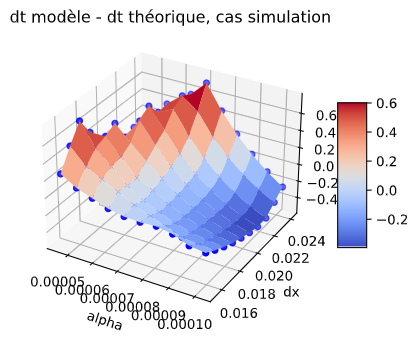
\includegraphics[width=0.7\textwidth]{surface-simulation.png}
    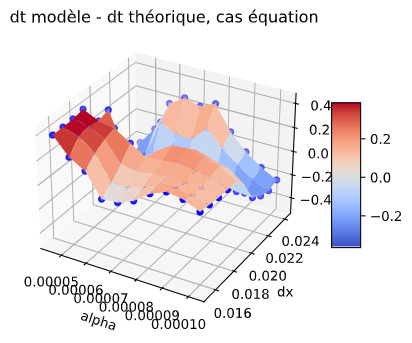
\includegraphics[width=0.7\textwidth]{surface-equation.png}
    \caption{Surfaces de comparaison des prédictions du réseau contre le résultat théorique.}
    \label{fig:correl}
\end{figure}

Dans la figure \ref{fig:surfaces} on montre les résultats de prédiction du réseau pour un ensemble aléatoire de valeurs de $\alpha$ et $dx$, dans les deux cas d'entraînement. On peut voir que pour les deux cas il existe des zones où le réseau donne des résultats au-dessus de la valeur théorique, ce qui n'est pas souhaitable, car ces valeurs ne donnent pas des schémas de discrétisation stables. 

% --------------------------------------------------------------
%                            Conclusion
% --------------------------------------------------------------

\section{Conclusion}

Dans le développement on a appris à approcher un problème d'apprentissage automatique lié à la discrétisation d'une EDP. Même si les résultats n'ont pas été idéales, on a pu conclure des points importants pour la suite.

D'un côté, on a vu que la maîtrise de la base données est un problème primordial pour un entraînement pertinent et précis. Cela veut dire qu'il faut (i) que le code qui la génère soit claire et pertinent, (ii) vérifier que les données générées sont correctes par rapport au problème en question, et pour cela caractériser statistiquement la base, et (iii) que la base ait une taille suffisante pour obtenir des résultats précis. Une faute dans cet aspect peut entraîner des difficultés en étapes postérieures ou des résultats erronés .

D'autre côté, il faut vérifier que l'entraînement du réseau soit ajusté aux contraintes du problème. On parle ici, par exemple et dans ce contexte-ci, de bornes sur les prédictions. Bien que la solution technique à ce problème reste comme tâche à réaliser, on a vu l'importance de cet aspect dans les résultats du réseau entraîné, car bien que les données de la base étaient toutes stables, le réseau résultant donne quand même des résultats instables. De ce fait, on peut conclure que ce type de conditions doivent être impliquées dans l'entraînement de quelque manière.
   

% --- Biblio par  bib
%\bibliography{ton-fichier-biblio}
%\bibliographystyle{plain-fr.bst}
%\selectlanguage{french}

%\begin{thebibliography}{7}
%\bibitem[Bastien 2019]{id-de-la-source}
%Auteurs : \emph{Un titre},  une date.
%\end{thebibliography}


% --------------------------------------------------------------
%                            Abstract
% --------------------------------------------------------------

\end{document}
